\graphicspath{{figure/chap1/}}
\chapter{波动光学基本原理}
\section{惠更斯原理}
惠更斯在距今三百多年前提出了一个关于光波传播的概念, 其大意如下:
光扰动同时到达的空间曲面被称为波阵面或者波前, 波前上的每一点都可以被看作一个新的扰动中心, 称其为子波源或次波源, 次波源向四周激发次波; 下一时刻的波前应当是这些大量次波面的公共切面, 也称其为包络面; 次波中心与其次波面上的那个切点的连线方向, 给出了该处光传播方向, 亦即光射线方向.

根据惠更斯原理, 人们可以由$t$时刻的波前, 用作图法导出下一时刻$t+\Delta t$的波前. 这个原理解决了波前随时间在空间中传播的问题.

\begin{figure}[htbp]
    \centering
    % 第一张图
    \begin{minipage}[b]{0.48\textwidth}
        \centering
        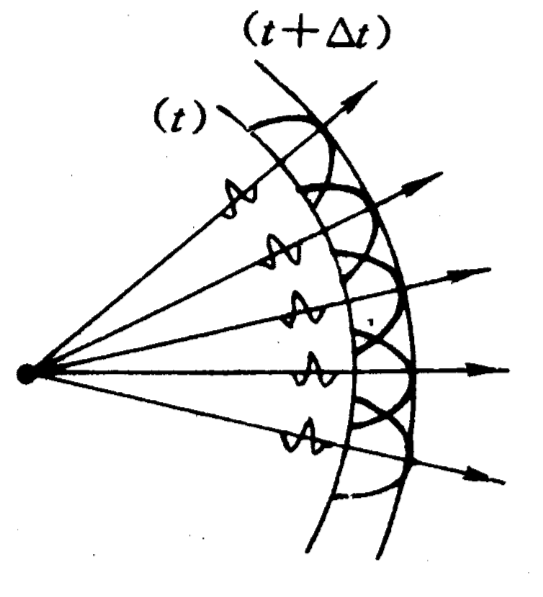
\includegraphics[width=0.55\textwidth]{1-1.png} % figure/image1.png
        \caption{均匀介质中光沿直线传播}
    \end{minipage}
    \hfill
    % 第二张图
    \begin{minipage}[b]{0.48\textwidth}
        \centering
        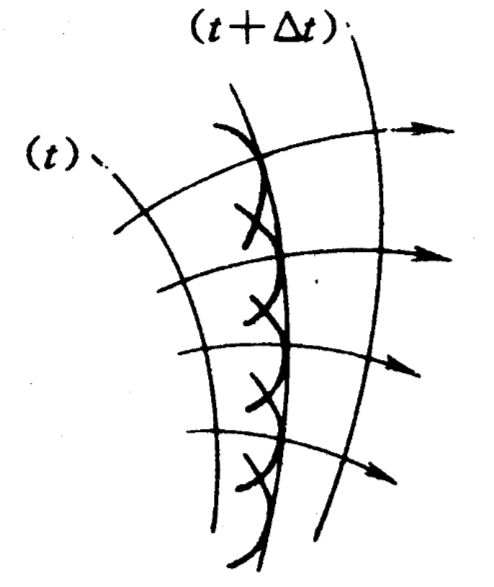
\includegraphics[width=0.55\textwidth]{1-2.png} % figure/image2.png
        \caption{非均匀介质中光线弯曲}
    \end{minipage}
\end{figure}

惠更斯原理可以得到一系列有意义的结果, 这里以折射定律为例说明. 如图, 设两种介质的界面为平面, 上方光速为$v_1$, 下方光速为$v_2$, 入射角为$i_1$. 取与入射光束正交的平面$ABC$作为波前, 则该波前上经过$C$点的光线到达入射点$C'$的时间为$\frac{CC'}{v_1}$. 以波前上的$A$点为次波源, 产生的次波的波面半径为$\rho_A=v_2 \Delta t$. 在$\Delta t$时间内, 波前上经过点$B$的光线传播到入射点$B'$后会有相应的按比例缩小的次波球面. 这样对次波球面作切线$C'A'$, 不难证明$C'A'$也相切于按比例缩小的一系列次波面上, 这就得到了一个存在于介质2中的新波前$C'B'A'$. 作新波前的法线, 这方向即为折射光线方向. 由几何关系可得:
\[
\sin i_1 = \frac{CC'}{AC} = \frac{v_1 \Delta t}{AC}, \quad \sin i_2 = \frac{AA'}{AC} = \frac{v_2 \Delta t}{AC}
\]
注意到$CC'=v_1\Delta t$,$AA'=v_2\Delta t$, 于是:
\[
\frac{\sin i_1}{\sin i_2} = \frac{v_1}{v_2}
\]

\insertfig{1-3.png}{由惠更斯原理导出折射定律}{0.35}

这样基于折射定律, 我们可以定义折射率$n$:
\[
\frac{\sin i_1}{\sin i_2} = n_{12} = \frac{n_2}{n_1}
\]

如果我们定义真空中的折射率为$1$, 则介质中的折射率为:
\[
n = \frac{c}{v}
\]

扰动在空间中传播而形成波动, 波速$v$等于扰动的时间频率$f$与波动的空间周期即波长$\lambda$的乘积, $v=f\lambda$. 设真空中的光速为$c=f_0\lambda_0$, 则折射率可以被表示为:
\[
n = \frac{f_0 \lambda_0}{f \lambda}
\]
问题是, 介质中光的频率$f$是否等于真空中的频率$f_0$? 在线性介质的光场中, 光扰动的时间频率仅由光源决定, 与介质无关. 这样我们有$f=f_0$, 折射率可以被简化为:
\[
n = \frac{\lambda_0}{\lambda}
\]
这表明在介质中光的波长变短了. 介质中的光的波长虽然变化, 其频率保持不变, 这也解释了为什么我们没有观察到介质中光的颜色变化, 因为真正与视网膜上视觉细胞相互作用的是光的扰动, 而决定扰动的时间频率是保持不变由光源决定的.

\section{费马原理}
我们定义光纤路径的几何长度与经过的介质折射率的乘积被定义为光程:
\[
L = \int_A^B n \d s
\]

光程的物理意义可以由下面的这个式子来说明. 考察一列由$A$传播到$B$的光波, 我们知道沿着光传播的方向, 各点扰动的相位是逐点落后的, 在单位长度上的相位落后由波数$k=\frac{2\pi}{\lambda}$决定, 即:
\[
\varphi(B)-\varphi(A) = -\int_A^{B}\frac{2\pi}{\lambda} \d s
\]
我们利用折射率的定义$n=\frac{\lambda_0}{\lambda}$, 可以将上式改写为:
\[
\varphi(B)-\varphi(A) = -\frac{2\pi }{\lambda_0}\int_A^B  n\d s = -\frac{2\pi}{\lambda_0} L
\]
这表明光程代表了光扰动在传播时的相位变化, 光程越大, 相位落后越多.

费马原理是说, 在光场中从$A$到$B$有一条实际光线$l_0$, 这个几何路径使得光程$L$取得平稳值:
\[
\int_{l_0} n \d s = \text{extreme}
\]

路径积分为平稳值, 有三种情况, 分别是取极小值---这最为常见; 取常数---成像时物像关系; 取极大值---这较为少见.

由费马原理可以导出直线传播定律, 反射定律和折射定律. 欧氏空间中两点间直线距离最短, 折射率为常数时显然应该沿此路径传播.

\begin{figure}[htbp]
    \centering
    % 第一张图
    \begin{minipage}[b]{0.48\textwidth}
        \centering
        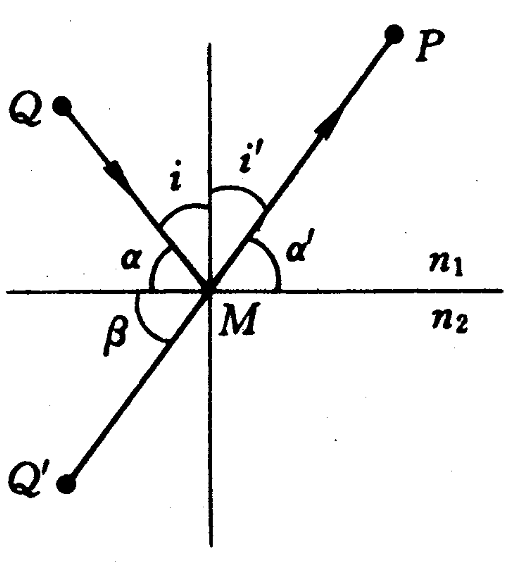
\includegraphics[width=0.55\textwidth]{1-4.png} % figure/image1.png
        \caption{费马原理导出反射定律}
    \end{minipage}
    \hfill
    % 第二张图
    \begin{minipage}[b]{0.48\textwidth}
        \centering
        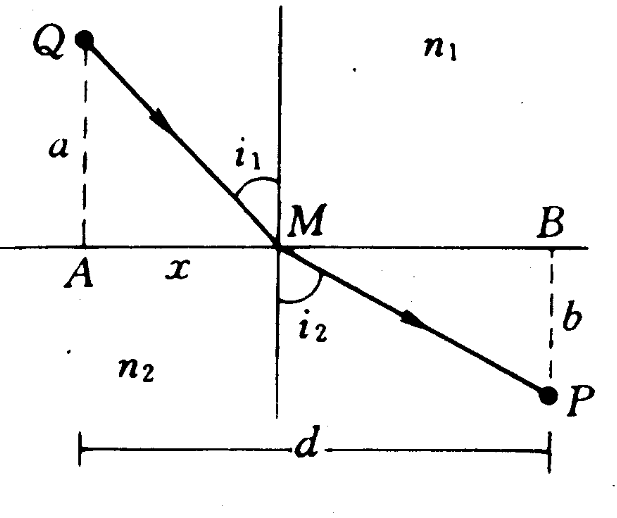
\includegraphics[width=0.55\textwidth]{1-5.png} % figure/image2.png
        \caption{费马原理导出折射定律}
    \end{minipage}
\end{figure}

对于反射情形, 引入光源关于反射面的镜面对称点$Q'$, 这样光程为极小值的条件显然是$Q'MP$为一条直线而非折线, 因此我们得到入射角等于反射角.

对于折射情形, 设定光源$Q$和观察点$P$, 界面上的动点$M$为待定的入射点, 考察光程:
\[
L(QMP) = n_1 QM + n_2 MP = n_1 \sqrt{a^2+x^2} + n_2 \sqrt{b^2+(d-x)^2}
\]

在这一元情况下取极值要求
\[
\frac{\d L}{\d x} = 0 \Rightarrow \frac{n_1 x}{\sqrt{a^2+x^2}} = \frac{n_2 (d-x)}{\sqrt{b^2+(d-x)^2}} \Rightarrow n_1 \sin i_1 = n_2 \sin i_2
\]

上式中已经利用
\[
    \sin i_1 = \frac{x}{\sqrt{a^2+x^2}}, \quad \sin i_2 = \frac{d-x}{\sqrt{b^2+(d-x)^2}}
\]

\begin{noteenv}
Richard Feynman 有更加独特的方式来看待镜面反射现象. Feynman 通过路径积分的方式利用许多小箭头解释了反射现象. Feynman提出, 光在参与反射时会经过所有可能的路径, 但镜子上的每一个点对于最终振幅的贡献是不一样的. 如图(a)所示, 我们将镜面分为许多方块, 每一个方块都对应着一条真实的光路. 显然这些光路对应的传播时间是不一样的. 现在让我们设想每个光子从光源出发时都携带了一块秒表, 其指针随着光的传播而转动, 初始时刻所有的秒表指针都指向同一方向, 在到达终点时停止计时, 这样箭头的方向就携带了相位信息. 我们用一系列箭头来代表各个方块对于最终的振幅贡献, 每个方块上的振幅大小相同, 因此各箭头的长度相同, 其方向如图(c)所示. 将他们叠加起来, 最终得到的结果如图(d)所示.

\begin{center}
\begin{minipage}[t]{0.48\linewidth}
    \centering
    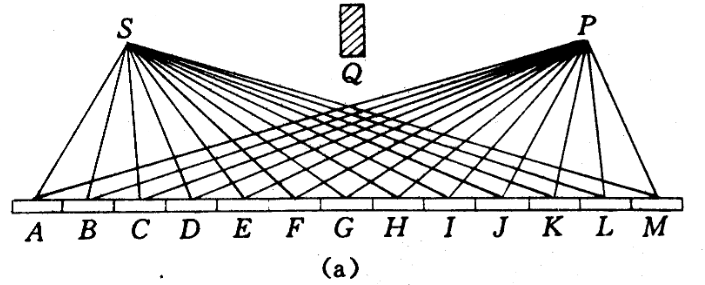
\includegraphics[width=\linewidth]{1-6.png}
\end{minipage}
\hfill
\begin{minipage}[t]{0.48\linewidth}
    \centering
    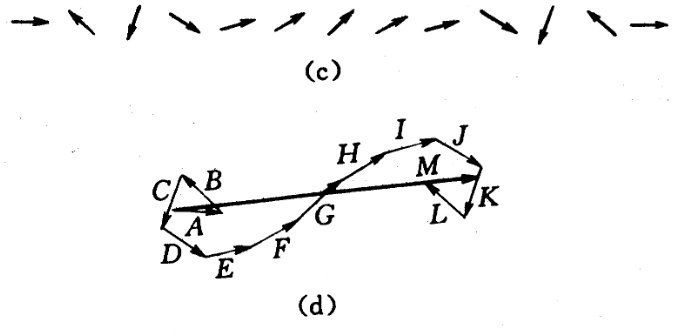
\includegraphics[width=\linewidth]{1-7.png}
\end{minipage}

\end{center}
我们发现对最终的振幅贡献最大的箭头位于中心, 这是因为此处光程取得极值, 相邻箭头间的方向变化不大, 相位差距不大, 叠加后仍有较大贡献. 而位于两端的相邻箭头间的相位差距较大, 导致它们的贡献相互抵消. 这样Feynman说, 费马原理指出的光程取稳定值是因为这条路径的及其邻近路径的光对于最终的振幅贡献最大. 这样的小箭头方法在我们处理衍射时也有一定意义.
\end{noteenv}

\section{光的叠加原理}
光是一种特定形式的电磁波, 可见光的波长$\lambda$约在$380\mathrm{nm}$到$760\mathrm{nm}$之间, 其对应的频率大约是$4 \times 10^{14}$到$8 \times 10^{14}$ Hz. Maxwell方程告诉我们, 各种形式的电磁波的传播速度都被波速方程制约为:
\[
v = \frac{1}{\sqrt{\mu \epsilon}} \Rightarrow n = \frac{c}{v} =  \frac{\sqrt{\mu \epsilon}}{\sqrt{\mu_0 \varepsilon_0}} = \sqrt{\varepsilon_r \mu_r}
\]

关于折射率的微观机制和性质的研究都是从上式出发的.

平面电磁波是自由空间电磁波的一个基元成分. 我们一般用电磁波的电场矢量来代表电磁波. 这样平面电磁波可以被表示为:
\[
\bm{E}(\bm{r}, t) = \bm{E}_0 \cos (\omega t - \bm{k} \cdot \bm{r}+\varphi_E)
\]

光是一种电磁波, 而电磁波是一种横波. 在与传播方向正交的平面上, $\bm{E}$和$\bm{H}$矢量的振动具有两个自由度, 这种平面上的方向自由度被称为光的偏振结构, 这也是偏振光的基础.

广义上说, 扰动在空间中的传播也就是运动状态在空间中的传播形成波动. 扰动同时到达的空间中各点形成一个等相位面. 按照等相位面的形状, 产生了各种对波的称谓, 例如平面波, 球面波等等.

按照时间尺度衡量, 波可以被分为定态波和脉冲波. 若在观测时间内光源持续且稳定地发光, 则波场中各点均以同一频率作稳定的振荡, 这种波被称为定态波. 而光源在极短时间中发光, 以至于波形局限于一个小区域内时, 这种波被称为脉冲波. 对于可见光, 其周期$T\approx 10^{-14}\mathrm{s}$, 普通光源从微观时间尺度看其一次持续发光时间量级$\tau\approx10^{-8} \mathrm{s}$. 一个长波列中大约含有$10^6$个周期, 这种情况就可以视为定态了. 发光的机制我们在讨论光的时间相干性时还会遇见.

现在我们考虑光波的相关叠加. 设在同一介质中有两列平面电磁波传播, 分别为:
\[
E_1 = \bm{E}_{10} \cos (\omega t - \bm{k}_1 \cdot \bm{r} + \varphi_1), \quad
E_2 = \bm{E}_{20} \cos (\omega t - \bm{k}_2 \cdot \bm{r} + \varphi_2)
\]

叠加后合成的光矢量为:
\[
E = E_1 + E_2 = \bm{E}_{10} \cos (\omega t - \bm{k}_1 \cdot \bm{r} + \varphi_1) + \bm{E}_{20} \cos (\omega t - \bm{k}_2 \cdot \bm{r} + \varphi_2)
\]

注意到能流密度矢量对时间取平均得到波的强度,
\[
I = \langle S \rangle = \frac{1}{2} c \varepsilon_0 n E_0^2 \propto E_0^2
\]

这样将上式两端对观察时间求平均得到:
\[
I = \langle \bm{E}^2 \rangle = \langle \bm{E}_1^2 \rangle + \langle \bm{E}_2^2 \rangle + 2\langle \bm{E}_1 \cdot \bm{E}_2 \rangle = I_1 + I_2 + 2\langle \bm{E}_1 \cdot \bm{E}_2 \rangle
\]
$2\langle\bm{E}_1 \cdot \bm{E}_2\rangle$被称为干涉项.

这里我们先不考虑偏振, 认为
\[
\bm{E}_1 \parallel \bm{E}_2
\]
从而我们可以写出干涉项的表达式为
\[
\begin{aligned}
2\langle \bm{E}_1 \cdot \bm{E}_2 \rangle & = 2 E_{10} E_{20} \langle \cos(\omega_1 t-\bm{k}_1\cdot \bm{r}_1+\varphi_{10})\cos(\omega_2 t -\bm{k}_2\cdot \bm{r}_2+\varphi_{20}) \rangle \\
& = E_{10}E_{20}\langle \cos((\omega_1+\omega_2) t -  (\varphi_{1} + \varphi_{2})) \rangle+ \langle \cos((\omega_1-\omega_2) t - (\varphi_{1} - \varphi_{2})) \rangle
\end{aligned}
\]
我们把光的空间传播带来的相位落后归结到$\varphi_1, \varphi_2$中. 上式中前一项取时间平均显然为零, 后一项在$\omega_1 = \omega_2$时不为零:
\[
2\langle \bm{E}_1 \cdot \bm{E}_2 \rangle = 2 E_{10} E_{20} \langle \cos(\Delta \varphi(P)) \rangle
\]
其中相位差$\Delta \varphi(P)$为
\[
\Delta \varphi(P) = \varphi_1 - \varphi_2 = \varphi_{10} - \varphi_{20}-k(r_1-r_2)
\]
这里把相位差写成场点$P$的函数意在强调正是相位差的空间变化决定了干涉条纹的形状和分布.

注意到只有在$\varphi_{10}-\varphi_{20}$恒定时, 对相位差的时间平均才不为零, 于是我们可以总结发生干涉的四个条件:
\begin{itemize}
    \item 光源的频率相同, 即$\omega_1 = \omega_2$.
    \item 光源的相位差$\varphi_{10} - \varphi_{20}$恒定.
    \item 两列光波的振动方向相同或有固定关系.
    \item 两列光波存在时空重叠.
\end{itemize}

对于取时间平均意义来说, 光源的相位差的绝对值并不重要, 不妨取$\varphi_{10}=\varphi_{20}$. 这样相位差可以被表示为:
\[
\Delta \varphi(P) = k(r_1 - r_2) = \frac{2\pi}{\lambda}(r_1 - r_2) = \frac{2\pi}{\lambda} \delta
\]
其中$\delta$为两列光波的光程差. 注意到:
\[
\Delta \varphi=
\begin{cases}
\pm 2k\pi, & \text{当 } \delta = k\lambda, k \in \mathbb{Z}, \cos(\Delta \varphi)= 1, \text{干涉光强极大} \\
\pm (2k-1)\pi, & \text{当 } \delta = (k-\frac{1}{2})\lambda,k\neq 0, k \in \mathbb{Z}, \cos(\Delta \varphi)= -1, \text{干涉光强极小} \\
\end{cases}
\]
考虑介质的折射率不为1时, 根据我们前面对光程的讨论, 我们可以得到:
\[
\Delta \varphi = \frac{2\pi}{\lambda} n (r_1 - r_2) = \frac{2\pi}{\lambda_n} (r_1 - r_2) = \frac{2\pi}{\lambda_n} \delta
\]
其中$\lambda_n = \frac{\lambda}{n}$是介质中的波长. 于是用波程差表达的干涉条件可以被写为:
\[
\begin{cases}
\delta = k \lambda_n, & k \in \mathbb{Z}, \quad \text{干涉极大} \\
\delta = (k - \frac{1}{2}) \lambda_n, & k \in \mathbb{Z}, \quad \text{干涉极小}
\end{cases}
\]


总结一下, 我们可以得到用光强表达的双光束干涉强度公式:
\[
I = I_1 + I_2 + 2\sqrt{I_1 I_2} \cos(\Delta \varphi(P))
\]

用振幅表达的双光束干涉强度公式:
\[
I = A_1^2 + A_2^2 + 2A_1 A_2 \cos(\Delta \varphi(P))
\]

用相位差表示的干涉条件:
\[
\begin{cases}
\Delta \varphi = 2k\pi, & k \in \mathbb{Z}, \quad \text{干涉极大} \\
\Delta \varphi = (2k-1)\pi, & k \neq 0, k \in \mathbb{Z}, \quad \text{干涉极小}
\end{cases}
\]

用波程差表示的干涉条件为:
\[
\begin{cases}
\delta = k \lambda_n, & k \in \mathbb{Z}, \quad \text{干涉极大} \\
\delta = (k - \frac{1}{2}) \lambda_n, & k \neq 0,k \in \mathbb{Z}, \quad \text{干涉极小}
\end{cases}
\]

